
\documentclass[11pt]{article}
\usepackage[margin=1in, top=15pt]{geometry}
\usepackage{amsmath, amssymb, xcolor, booktabs, graphicx,  enumitem}

% for graphs
\usepackage{tikz}
\usetikzlibrary{graphs, graphs.standard, quotes}

\title{CS 225}
\author{Some ways to draw graphs}
\date{Fall 2020}

\begin{document}
\maketitle
\hrule

\bigskip
\section*{Include the graph as a picture:}

\includegraphics[scale=0.3]{graphs_updated.png}

\section*{Use Tikz with the graph library}

Need to put ``{$\backslash$}usepackage\{tikz\}'' then ``{$\backslash$}usetikzlibrary\{graphs, graphs.standard, 
quotes\}'' into preamble. 

% vertices not in a line
\begin{center}
    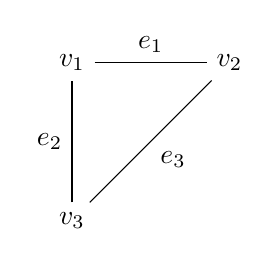
\begin{tikzpicture} 
        % the math nodes option makes it so it interprets the name of the node (vertex)
        % as in math mode, and the name also becomes the label of the vertex

        % I know how to make it draw vertices as points (this is in the tikz documentation), 
        % but I don't know how to make the tikz library graphs with vertices as 
        % points and labels below the points. 

        % the number for grow right seems to determine horizontal spacing of vertices
        % the number for branch down seems to determine vertical spacing of vertices
        \graph[math nodes, grow right=2cm, branch down=2cm] {
            % the -- denotes an edge 
            % information in the [] after an edge determines options
            % I think this way of labeling uses the quotes tikz library
            v_1 -- ["$e_1$"] v_2;
            v_3 -- ["$e_2$"] v_1;
            % the swap option puts the label on the other side of the edge
            v_3 -- ["$e_3$", swap] v_2;
        };
    \end{tikzpicture}
\end{center}

% linear graph
\begin{center}
    \begin{tikzpicture}
        \graph[math nodes, grow right=2cm, branch down=2cm] {
            v_1 -- ["$e_1$"] v_2;
        };
    \end{tikzpicture} 
\end{center}

% loop
\begin{center}
    \begin{tikzpicture}
        \graph[math nodes, grow right=2cm, branch down=2cm] {
        % use the loop option for an edge from a vertex to itself to get a loop
        % I don't know how to make it not directed
        v_1 -- ["$e_1$", loop, swap] v_1;
        };
    \end{tikzpicture}
\end{center}

% parallel edges
\begin{center}
    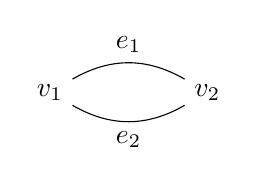
\begin{tikzpicture}
        \graph[math nodes, grow right=2cm, branch down=2cm] {
        % bend left bends the edge left (left as you travel from the first vertex to the next)
        % there is also a way to specify how far it bends left
        v_1 -- ["$e_1$", bend left] v_2;
        v_1 -- ["$e_2$", bend right, swap] v_2;
        };
    \end{tikzpicture}
\end{center}

\end{document}